\documentclass[a4paper]{article}

\usepackage{xcolor}
\usepackage{fancyheadings}
\usepackage{listings}
\usepackage{graphicx}
\usepackage[utf8]{inputenc}
\usepackage{multirow}
\lstset{frameround=fttt,numbers=left,breaklines=true, extendedchars=true}

\newcommand{\todo}[1]{\textcolor{red}{[#1]}}
\lhead{Open Universiteit}
\chead{IM0202, Software evolution}
\rhead{Assignment 1}

\begin{document}
\pagestyle{fancy}

\section*{Studentgegevens}
\begin{description}
	\item [Cursuscode] IM0202
	\item [Naam] Ewoud Westerbaan
	\item [Studentnummer] 852069942
	\item [Naam] Martin de Boer
	\item [Studentnummer] 837372832
\end{description}

\section*{Samenwerking}
Nadat Ewoud een git repository had aangemaakt voor het rascal
project, zijn we beide begonnen aan een eigen module. De modules
zijn parallel aan elkaar ontwikkeld, zodat er redelijk
zelfstandig kon worden gewerkt. In grote lijnen heeft Ewoud de
modules \texttt{metrics::Volume.rsc} en
\texttt{metrics::Duplicates.rsc} voor zijn rekening genomen, en
Martin de modules \texttt{metrics::UnitSize.rsc} en
\texttt{metrics::Complexity.rsc}.

De module \texttt{metrics::Volume.rsc} berekent het aantal lines
of code (LOC). \texttt{metrics::UnitSize.rsc} doet hetzelfde
voor de units (methodes en constructoren) in het project. De
module \texttt{metrics::Duplicates.rsc} zoekt naar dubbele code
in het project. En de module \texttt{metrics::Complexity.rsc},
tenslotte, bepaalt per unit (methode/constructor) de complexity
measure.

Bepaalde code leende zich voor hergebruik, en daarvoor is in
samenspraak een module \texttt{utils::Utils} in het leven
geroepen, waaraan beide auteurs hebben gewerkt.

Martin heeft tijdens het ontwikkelen van de modules een eerste
opzet gemaakt voor het unittesten van de modules. Het
inhoudelijk schrijven van de testcode is op dezelfde wijze
verdeeld als de modules zelf: beide auteurs hebben de testcode
voor hun eigen modules geschreven. Voor het testen is er wat
intensiever samengewerkt, ook omdat daarbij aanvankelijk wat
technische probleempjes optraden.

\section{Aannames}
\subsection{Duplicaten}
In onze oplossing vergelijken we de content van methodes en constructoren met elkaar, maar dit gebeurt in één richting. Als methode A wordt vergeleken met methode B, wordt methode B niet meer vergeleken met methode A. Stel dat het aantal opeenvolgende regels dat identiek is, 6 is. Dan is de duplicatiewaarde over de oplossing dus 6 / 12, dus 50\%. Als we dan drie methodes gebruiken, dan wordt methode A met methode B vergeleken, methode A met methode C én methode B en methode C. Het aantal duplicate regels is dan 18, wat gelijk is aan het totaal van aantal regels. In figuur \ref{fig:DuplicatenDetectie} hebben we dit doorgetrokken. op de x as staan het aantal methodes dat dezelfde code bevat. De blauwe lijn geeft het totaal aantal regels code in de oplossing aan, en de rode lijn het aantal gedetecteerde duplicate regels. Het aantal duplicate regels loopt dus exponentieel.
\begin{figure}[htbp]
\caption{Oplopen van detectieregels bij meerdere methodes}
\centering
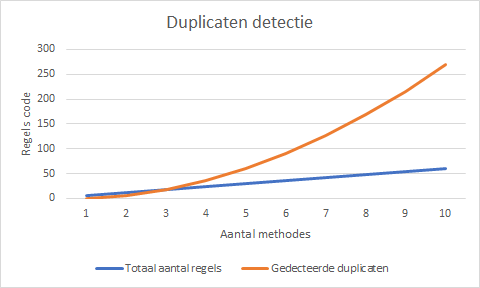
\includegraphics[width=0.8 \textwidth]{DuplicatenDetectie.png}
\label{fig:DuplicatenDetectie}
\end{figure}
Onze aanname is dat het aantal duplicate regels het totaal van regels is dat meerdere keren in de applicatie voorkomt. Dit hebben wij geimplementeerd door de set van unitparen te verdelen over sets gegeven het aantal duplicate regels. Van deze set maken wij een set van 2-tuples waarbij we de locatie en het startnummer binnen de content concateneren. Vervolgens beschouwen we deze nieuwe relatie als een graaf waarbij we het aantal units vermenigvuldigen met het aantal duplicate regels.

Ter verduidelijking: laten we aannemen dat we 4 gelijke methodes hebben van 6 regels code. Als we voorheen de duplicatie berekende, kregen we 6 onderlinge verbindingen maal 6 regels duplicate code is 36 regels (van de 24 in totaal). Met de bovenbeschreven methode krijgen we dan een groep van 4 elementen. Dit maal 6 regels duplicate code levert 24 op.

Op deze manier zal ook een enkele duplicaat (dus 2 units dat dezelfde code bevatten) geen 50\% score opleveren, maar 100\%. Dat zagen we ook terug in het draaien met de verschillende vormen over het testobject (SmallSQL); voorheen hadden we een score van 4,5\%, maar met de laatste vorm een score van ongeveer 12\%.

\subsection{Unitsize versus volume}
We zien een verschil in de som van de unitsize ten opzicht van het volume. Wij beschouwen het volume als alle regels code in een java file, zonder commentaar en zonder de lege ruimtes, zoals ook in \cite{A}. \texttt{Import} statements en field definitions beschouwen wij als ook onderdeel van het volume. De som van de regels code daarentegen, is de som van de inhoud van de methodes en contructoren (de units). Omdat de complexiteit en duplicaten berekend worden over de inhoud van de units, gebruiken wij deze metriek om het duplicaat en de complexiteit percentage te berekenen.

\subsection{Lines of code}
Gedurende het project zijn we 
overgestapt naar een andere
signature van methode locaties. 
In het begin van het project was
een locatie bijvoorbeeld
\begin{lstlisting}
|java+method:///DuplicationTestClass/duplicationTestLastPartEquals_ExpectTrue()|
\end{lstlisting}
later is dit veranderd naar
\begin{lstlisting}
|project://DuplicationTest/src/DuplicationTestClass.java|(1085,260,<42,49>,<51,2>)
\end{lstlisting}
Dit had invloed op de content die met elkaar vergeleken werd.
Deze locaties zijn te krijgen door de \texttt{getUnits()} aan te
roepen in de module \texttt{utils::Utils}. Met de eerste
locatie, was de content die eruit gehaald werd inclusief de
method (of constructor) signature (bijvoorbeeld: \texttt{public
int getNumber()}). Op de tweede manier begint de content die
opgehaald worden met de accolade (\texttt{\{}) achter de method
signature. Met de regressie testen van de duplicaten, blijkt dus
dat het aantal gelijke regels overal met 1 was toegenomen. De vraag die nu opspeelt is: moeten we de methode signatures ook zien als code dat vergeleken moet worden. Echter, duplicatie gaat over code in de code-blocks \cite{A}. Wij besluiten daarom dat de method signature daar niet onder valt. De accolades waarmee de methode start en eind moeten dus verwijderd worden bij het schoonmaken van de content (trimmen van de content en het verwijderen van commentaar).

De versie van locatie waar we naar overgestapt zijn, had grote invloed op onze unittests. Deze waren heel gevoelig voor wijzigingen omdat deze op character niveau keken naar de locatie.

De lines of code zijn belangrijk voor de metrieken volume en unitsize. Beiden
maken gebruik van regels code die geen commentaar zijn. Omdat
dit een gemeenschappelijke logica is, is deze gedefinieerd in de
\texttt{utils::Utils} module.
Regels code worden nu beschouwd als alle niet lege regels minus
de commentaar regels. Dit `schoonmaken' van de inhoud van een unit wordt ook gebruikt voor controle op duplicaten.

\subsection{Complexity}
De complexiteitsmaat heeft betrekking op het aantal paden die in
een unit (methode of constructor) kan worden bewandeld. Dit zegt
iets over de testbaarheid van zo'n unit. We gaan er vanuit dat
de standaard complexiteitsmaat de waarde 1 heeft, en dat er voor
een aantal taaconstructies reden is om deze met 1 te verhogen.
Deze taalconstructies blijken duidelijk uit de onderstaande
code:

\begin{lstlisting}[caption={Taalsconstructies die de
complexiteit verhogen},label={lst:complexity},escapechar=|,
frame = single]
int complexity = 1;
visit(stat) {
  case \case(_) : complexity += 1;
  case \do(_, _) : complexity += 1;
  case \if(_, _) : complexity += 1;
  case \catch(_,_): complexity += 1;
  case \while(_, _) : complexity += 1;
  case \if(_, _, _) : complexity += 1;
  case \for(_, _, _) : complexity += 1;
  case infix(_,"&&",_) : complexity += 1;
  case infix(_,"||",_) : complexity += 1;    
  case \for(_, _, _, _) : complexity += 1;
  case \foreach(_, _, _) : complexity += 1;
  case \conditional(_,_,_): complexity += 1;
}
\end{lstlisting}

De \texttt{if}-constructies spreken voor zich: de conditie kan
waar zijn of niet. Er zijn dus twee mogelijkheden, waarmee het
aantal mogelijke paden met 1 wordt uitgebreid. Ditzelfde geldt
voor de \texttt{conditional} in Java (feitelijk een alternatieve
manier van het schrijven van een if-constructie, bijv.:
\texttt{b == true ? x : y;}). De \texttt{do}, \texttt{while},
\texttt{for}, en \texttt{foreach} be\"invloeden de complexiteit
op een vergelijkbare manier. In het \texttt{switch}-statement,
is iedere \texttt{case} te beschouwen als een
\texttt{if}-statement, en dus verhogen we voor iedere
\texttt{case} de complexiteitsmaat met 1.
De \texttt{default}-tak voegt wel een extra stap, maar geen
extra pad aan de sequentie van statements toe, en heeft dus geen
invoed op de complexiteitsmaat.
Het optreden van een exception kan worden afgehandeld in een
\texttt{catch}-blok. Ieder \texttt{catch}-blok voegt een nieuw
pad aan de control-flow van het programma toe, zodat ook dit de
complexiteit verhoogd.
Tenslotte is er de infix-notatie (AND, of OR-variant) die
invloed heeft op het aantal paden. We verhogen hiervoor de de
complexiteitsmaat wederom met 1, omdat het al dan niet
\texttt{true} zijn van de linker-conditie bepaald of de tweede
conditie wordt bepaald.



\section{Resultaten}
In Listing \ref{lst:output} is de output van het geschreven programma te zien over SmallSQL. 

\begin{lstlisting}[caption={Programma output SmallSQL},label={lst:output},frame = single]
Volume berekenen ...
Berekend volume: 
- totaal aantal regels (incl. lege regels): 35271
- commentaarregels: 4102
- coderegels: 22192

Unit size berekenen ...
Aantal gevonden units (methodes en constructoren): 2494
Som van de aantallen regels per methode/constructor:
- totaal aantal regels (incl lege regels binnen de units): 22730
- commentaarregels: 628
- coderegels: 16401

Berekenen cyclomatische complexiteit ...

Aggregeren gegevens (unit size and complexity) ...
- Categorie Simple (Without much risk): 67%
- Categorie Moderate (With moderate risk): 10%
- Categorie Untestable (Untestable, very high risk): 7%
- Categorie Complex (Complex, with high risk): 14%
- Rank op basis van aggregatie: --

Berekenen duplicatie ...
size of pairs to check: 203203
- Aantal duplicaties: 188
- Aantal regels gedupliceerd: 1976
- Duplicatepercentage: 12.04804585%

Programma beeindigd
\end{lstlisting}
 
\section{Betrouwbaarheid}
De betrouwbaaheid en de juistheid van de oplossing kunnen we waarborgen door het gebruik van unittests. 
We hebben meerdere `dummy'-projecten gemaakt die dienen als referentieproject bij het draaien van deze tests. 
Door dat we zelf deze projecten maken, welke klein en overzichtelijk zijn, kunnen we vrij specifiek meten, testen en de juistheid valideren van de opgeleverde code. In Listing \ref{lst:testoutput} is de output weergegeven van onze unittests.
\begin{lstlisting}[caption={Unit test output},label={lst:testoutput},frame = single]
Running tests for tests::metrics::DuplicationTest
Test report for tests::metrics::DuplicationTest
        all 13/13 tests succeeded
Running tests for tests::metrics::VolumeTest
Test report for tests::metrics::VolumeTest
        all 3/3 tests succeeded
Running tests for tests::metrics::UnitSizeTest
Test report for tests::metrics::UnitSizeTest
        all 2/2 tests succeeded
Running tests for tests::metrics::AggregateTest
Test report for tests::metrics::AggregateTest
        all 1/1 tests succeeded
Running tests for tests::utils::TestUtilsTest
| testing 0/5 Test failed. Msg: ** No worries! This test should fail **. Expected = blabla, actual = bla
Test failed. Msg: ** No worries! This test should fail **. Expected = 1, actual = 2
Test report for tests::utils::TestUtilsTest
        all 5/5 tests succeeded
Running tests for tests::metrics::RateTest
Test report for tests::metrics::RateTest
        all 11/11 tests succeeded
Running tests for tests::utils::UtilsTest
Test report for tests::utils::UtilsTest
        all 18/18 tests succeeded
Running tests for tests::metrics::ComplexityTest
Test report for tests::metrics::ComplexityTest
        all 2/2 tests succeeded
bool: true
\end{lstlisting}
\section{Interpretatie}
Als we de output van \ref{lst:output} nemen en deze tegen de referentie tabellen aanhouden als in \cite{A}, kunnen we een soortgelijk resultatentabel invullen. Omdat wij unittesting niet gemeten hebben, laten we deze buiten beschouwing.

De output van het programma (Listing \ref{lst:output}) geeft voor volume 22192 code regels. Dit geeft een rank van ++.

Voor de complexity hebben we het percentage berekent per categorie. Als we de rank hiervan opzoeken, komen we op - - (2x -).

Het duplicatiepercentage is 12.04\%. Dat kunnen we vertalen met het rating schema naar een enkele -.

Voor de interpretatie van de unitsizes zijn door \cite{A} geen strikte waardes gegeven, daarom dienen wij hier zelf een methode voor te bedenken.
Eerst classificeren wij de units door middel van Tabel \ref{tbl:UnitSizeClassificatie}.

\begin{table}[h]
\caption{Unitsize classificatie}
\label{tbl:UnitSizeClassificatie}
\begin{tabular}{|l|l|}
\hline
Unitsize         & Classificatie      \\ \hline
1-5              & small units        \\
6-15             & medium sized units \\
16-25            & large units        \\
\textgreater{}25 & very large units   \\ \hline
\end{tabular}
\end{table}

Met de relatieve aantallen ten opzichte van het toaal aantal units, geven we de applicatie een ranking, zoals we deze in Tabel \ref{tbl:UnitsizeRanking} hebben weergegeven.

\begin{table}[h]
\caption{Unitsize ranking}
\label{tbl:UnitsizeRanking}
\begin{tabular}{cl|lll|}
\cline{3-5}
\multicolumn{1}{l}{}       &  & \multicolumn{3}{c|}{maximum relative units}                                              \\ \hline
\multicolumn{1}{|c|}{rank} &  & \multicolumn{1}{c}{moderate} & \multicolumn{1}{c}{high} & \multicolumn{1}{c|}{very high} \\ \hline
\multicolumn{1}{|c|}{++}   &  & \multicolumn{1}{c}{20\%}     & \multicolumn{1}{c}{0\%}  & \multicolumn{1}{c|}{0\%}       \\
\multicolumn{1}{|c|}{+}    &  & \multicolumn{1}{c}{30\%}     & \multicolumn{1}{c}{5\%}  & \multicolumn{1}{c|}{0\%}       \\
\multicolumn{1}{|c|}{o}    &  & \multicolumn{1}{c}{40\%}     & \multicolumn{1}{c}{10\%} & \multicolumn{1}{c|}{0\%}       \\
\multicolumn{1}{|c|}{-}    &  & \multicolumn{1}{c}{50\%}     & \multicolumn{1}{c}{15\%} & \multicolumn{1}{c|}{5\%}       \\
\multicolumn{1}{|c|}{--}   &  & \multicolumn{1}{c}{-}        & \multicolumn{1}{c}{-}    & \multicolumn{1}{c|}{-}         \\ \hline
\end{tabular}
\end{table}

Het resulaat is dat unitsize van ons een score krijgt van \todo{waarde invullen}.

Als we alle waardes in de tabel zetten zoals in \cite{A}, komen we uit op Tabel \ref{tbl:ResultaatSmallSQL}. De laatste kolom hiervan lichten we toe.
\begin{description}
\item[Analysability] \todo{blablabla}
\item[Changeability] Omdat de complexity per unit zeer hoog is, en de hoeveelheid duplicatie ook vrij hoog is, geven we changeability de score -.
\item[Stability] We hebben de waarde van de unit testing niet gemeten. Hierdoor kunnen we niets zeggen over de stability en krijgt deze de neutrale waarde `o'.
\item[Testability] Omdat we unit testing niet hebben gemeten, is de testability volledig afhankelijk van de complexity per unit. Deze is voor SmallSQL zeer hoog en daarom geven we testability de gelijke waarde als complexity per unit: - -.
\end{description}
\begin{table}[h]
\caption{Resultaat SmallSQL}
\label{tbl:ResultaatSmallSQL}
\begin{tabular}{llllllll}
                          &                                                      &                                    & \multicolumn{5}{l}{source code properties}                                                                                                                           \\ \cline{4-7}
                          &                                                      & \multicolumn{1}{l|}{}              & \multicolumn{1}{c|}{\rotatebox[origin=c]{90}{volume}} & \multicolumn{1}{c|}{\rotatebox[origin=c]{90}{ complexity per unit }} & \multicolumn{1}{c|}{\rotatebox[origin=c]{90}{duplication}} & \multicolumn{1}{c|}{\rotatebox[origin=c]{90}{unit size}} &                         \\ \cline{4-7}
                          &                                                      & \multicolumn{1}{l|}{}              & \multicolumn{1}{c|}{++}       & \multicolumn{1}{c|}{- -}                    & \multicolumn{1}{c|}{-}            & \multicolumn{1}{l|}{}          &                         \\ \cline{3-8} 
\multirow{4}{*}{\rotatebox[origin=c]{90}{ISO 9128}} & \multicolumn{1}{l|}{\multirow{4}{*}{\rotatebox[origin=c]{90}{maintainablity}}} & \multicolumn{1}{l|}{analysability} & \multicolumn{1}{c|}{X}      & \multicolumn{1}{l|}{}                    & \multicolumn{1}{c|}{X}           & \multicolumn{1}{c|}{X}         & \multicolumn{1}{c|}{???} \\ \cline{3-8} 
                          & \multicolumn{1}{l|}{}                                & \multicolumn{1}{l|}{changeability} & \multicolumn{1}{l|}{}       & \multicolumn{1}{c|}{X}                   & \multicolumn{1}{c|}{X}           & \multicolumn{1}{l|}{}          & \multicolumn{1}{c|}{- -} \\ \cline{3-8} 
                          & \multicolumn{1}{l|}{}                                & \multicolumn{1}{l|}{stability}     & \multicolumn{1}{l|}{}       & \multicolumn{1}{c|}{}                    & \multicolumn{1}{l|}{}            & \multicolumn{1}{l|}{}          & \multicolumn{1}{c|}{0} \\ \cline{3-8} 
                          & \multicolumn{1}{l|}{}                                & \multicolumn{1}{l|}{testability}   & \multicolumn{1}{l|}{}       & \multicolumn{1}{c|}{X}                   & \multicolumn{1}{l|}{}            & \multicolumn{1}{l|}{}          & \multicolumn{1}{c|}{- -} \\ \cline{3-8} 
\end{tabular}
\end{table}

\bibliographystyle{abbrv}
\bibliography{verslag_assignment1}

\end{document}
